\documentclass[a4paper, 12pt, titlepage]{article}
%=======Unpackage Things===============
\usepackage{color}
\usepackage{colortbl}
\usepackage{mathrsfs}

\usepackage{graphicx}
\usepackage{amsthm}
\usepackage{listings}
%\usepackage{fullpage}
\usepackage{epsfig}
\usepackage{amsmath}
\usepackage{latexsym}
\usepackage{amssymb}
\usepackage{amstext}
\usepackage{array}
\usepackage{titlesec}
\usepackage{float}

\titleformat{\section}
    {\normalfont\fontsize{12}{15}\bfseries}{\thesection}
    {1em}{}
\newcommand{\PreserveBackslash}[1]{\let\temp=\\#1\let\\=\temp}
\newcolumntype{C}[1]{>{\PreserveBackslash\centering}p{#1}}
\newcolumntype{R}[1]{>{\PreserveBackslash\raggedleft}p{#1}}
\newcolumntype{L}[1]{>{\PreserveBackslash\raggedright}p{#1}}


\begin{document}
%==title==
\title{COMP6321 Assignment 2}
\setcounter{tocdepth}{2}
\newpage
\begin{center}
    {\huge COMP6321: Assignment \#2}


    \vspace{2cm}
    Student: Qing Gu  \hspace{5cm}
    Student ID: 6935451
    \vspace{1cm}

    =================================================
\end{center}
\section{L1 vs. L2 Regularization}
\begin{enumerate}
    \item Assume the training data follows i.i.d. I use first 80 data for training and last 9 data for testing. In order to adopt L2 regression, we have to change the cost function to:
        $$J(w) = \frac{1}{2}(\phi{}w-y)^T(\phi{}w-y)+\frac{\lambda}{2}w^Tw$$
        $$w^* = (\phi^T\phi+\lambda{}I)^{-1}\phi^Ty$$
        The root mean squared error and weights are ploted in fig~\ref{l2err} and fig~\ref{l2weight}.

            \begin{figure}[H]
                \centering
                \includegraphics[width=8cm]{L2Err.eps}
                \caption{L2 Regression Errors}\label{l2err}
            \end{figure}

            \begin{figure}[H]
                \centering
                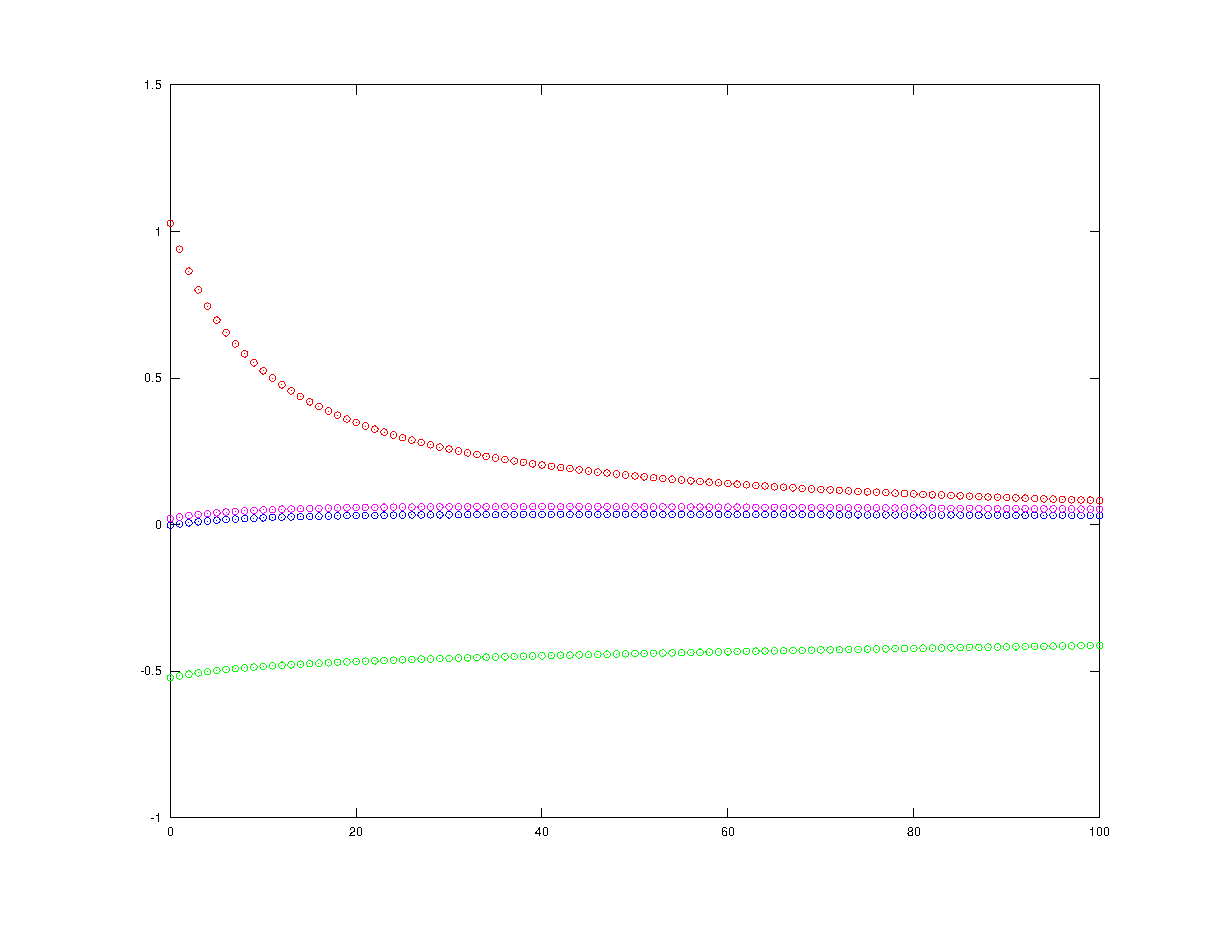
\includegraphics[width=8cm]{L2Weight.eps}
                \caption{L2 Regression Errors}\label{l2weight}
            \end{figure}

            
        
    \item For this data set, we have 4 weights to deal with. Thus, the L2 problem is:
        $$\min_{w1, w2, w3} \sum^m_{j=1}(y_j-w_1x_1-w_2x_2-w_3x_3)$$
        where
        $$|w_1, w_2, w_3|<\lambda$$
        In order to adopt quadratic programming:
        $$J(w) = \frac{1}{2} w^THw + f^Tw subject to Aw\leq{}b$$
        where
        $$H = X^TX, f=-(y^TX)^T, b=\lambda$$
        \[A=
        \left|
        {\begin{array}{ccc}
                1 & 1 & 1\\
                1 & 1 & -1\\
                1 & -1 & 1\\
                -1 & 1 & 1\\
                -1 & -1 & 1\\
                -1 & 1 & -1\\
                1 & -1 & -1\\
                -1 & -1 & -1\\
        \end{array}}
        \right|
        \]
    \item Root mean squared errors and weights are plotted in fig~\ref{l1err} and~\ref{l1weight}.

            \begin{figure}[H]
                \centering
                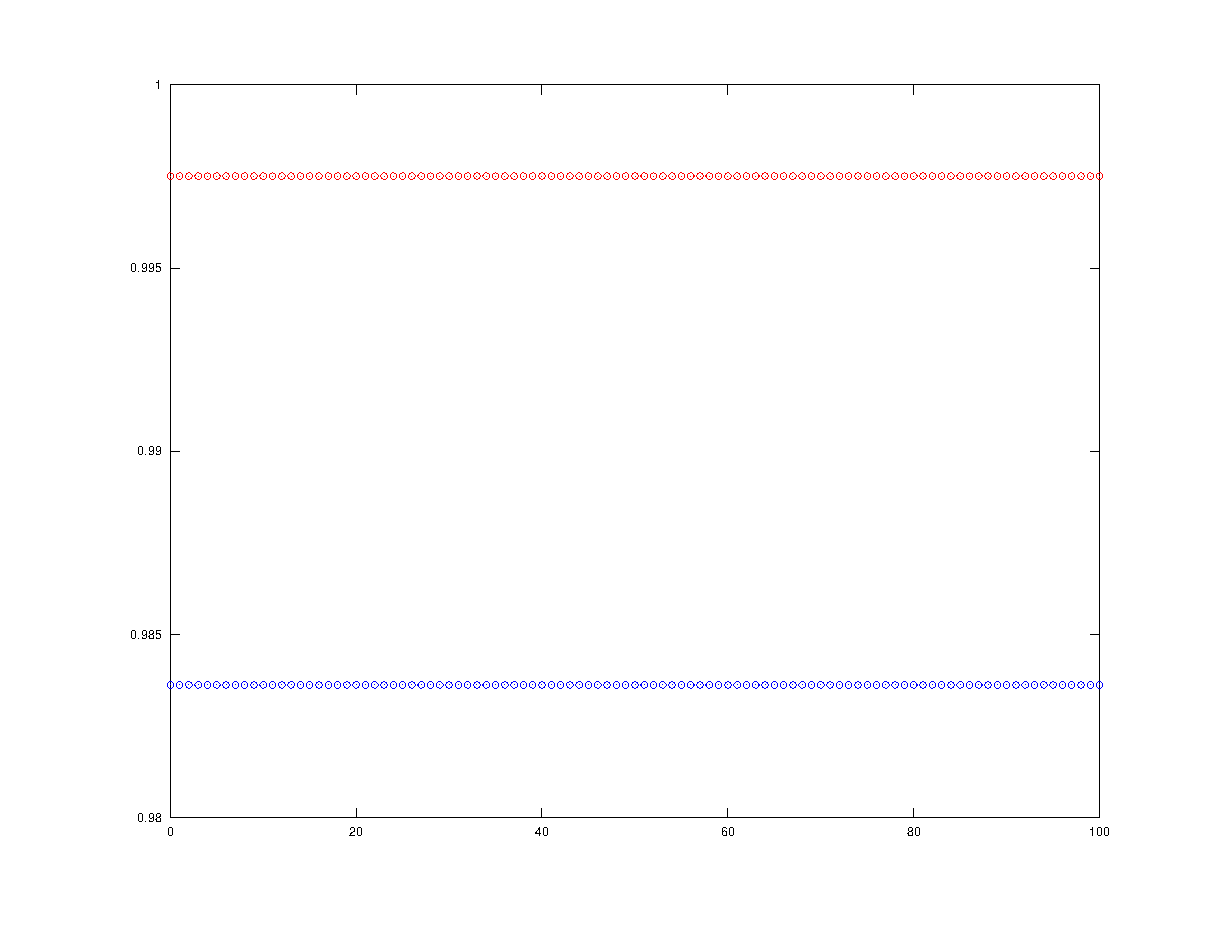
\includegraphics[width=8cm]{L1Err.eps}
                \caption{L2 Regression Errors}\label{l1err}
            \end{figure}

            \begin{figure}[H]
                \centering
                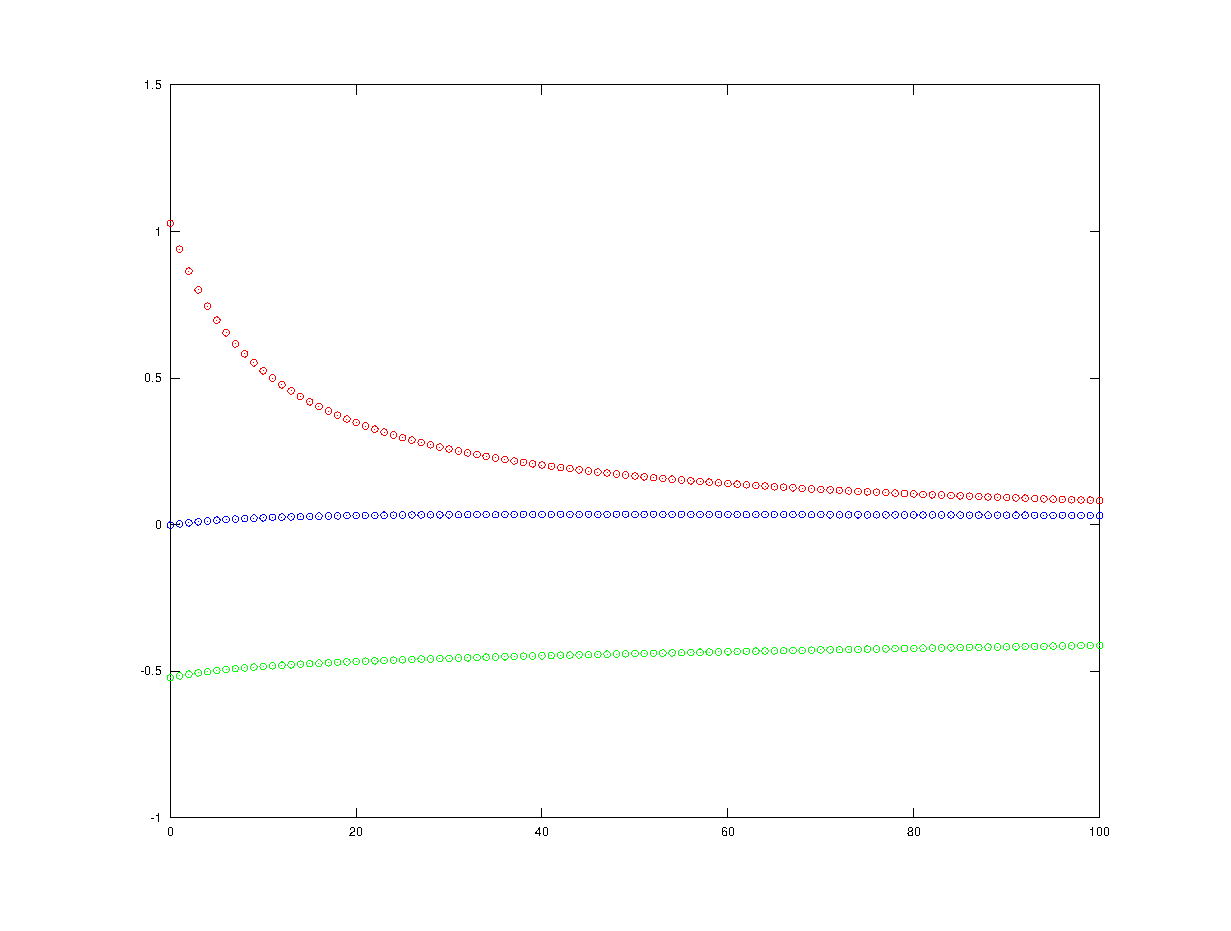
\includegraphics[width=8cm]{L1Weight.eps}
                \caption{L2 Regression Errors}\label{l1weight}
            \end{figure}

            L1 regularization is expected to be better when we have more features than trainig examples. However, when we have enough trainig data, L2 regularization is better.
\end{enumerate}

\section{Dealing with Missing Data}

The goal of generative learning is to calculate the posterior $P(y|x)$ with an application of Baye's Rule and access to prior $\pi=P(y=1)$ and the liklikhhod of both classes( i.e $P(x|y=0)$ and $P(x|y=1)$).
Using the Baye's rule, we have:
$$P(Y=1|x) = \frac{P(x|y=1)P(y=1)}{p(X)}$$
Since the tow classes are modeled as:
$$P(x|y=0) = \frac{1}{(2\pi)^{n/2}|\Sigma|^{1/2}}\exp{(-\frac{1}{2}(x-\mu_0)^T\Sigma^{-1}(x-\mu_0))}$$
$$P(x|y=1) = \frac{1}{(2\pi)^{n/2}|\Sigma|^{1/2}}\exp{(-\frac{1}{2}(x-\mu_1)^T\Sigma^{-1}(x-\mu_1))}$$
The function can be rewrite:
$$P(y=1|x) = \frac{1}{1+e^{-(\mu_1-\mu_0)^T\Sigma^{-1}(x-frac{\mu_0+\mu_1}{2})+\log\frac{1-\pi}{\pi}}}$$

In this problem, we have $x_n$ lost and have $E(x_n|y=0)$ and $E(x_n|y=1$, i.e. $\mu_0$ and $\mu_1$ filled. Obviously, the filled data will not change $\mu_0, \mu_1, \Sigma$ and $\pi$, thus the prediction will not change.

\section{Naive Bayes Assumption}

\begin{enumerate}
    \item The initial Naive Bayes classifier should have 5 paramters, i.e. $\theta_1, \theta_{1,0}, \theta_{2, 0}, \theta_{1, 1}, \theta_{2, 1}$. There are 7 parameters for classifier with 3 features, they are $\theta_1, \theta_{1,0}, \theta_{2, 0},\theta_{3, 0}, \theta_{1, 1}, \theta_{2, 1}$ and $\theta_{3, 1}$
    \item In this example, we have feature $x_2$ and $x_3$ duplicated. $\theta_{2,1}, \theta_{2,0}$ and $\theta_{3,1}, \theta_{3,0}$ should be identical if the model is perfectly learnt. Put it into the descion surface:
        $$\frac{P(y=1|x)}{P(y=0|x)}=\frac{P(y=1)\Pi^3_{i=1}\theta^{x_i}_{i,1}(1-\theta_{i,1})^{1-x_i}}{P(y=0)\Pi^3_{i=1}\theta^{x_i}_{i,0}(1-\theta_{i,0})^{1-x_i}}$$
        Using the log trick:
        $$\log{\frac{P(y=1|x)}{P(y=0|x)}}=\log{\frac{P(y=1)_i}{P(y=0}} + \log{\frac{P(x_1|y=1)}{P(x_1|y=0)}}+\log{\frac{P(x_2|y=1)}{P(x_2|y=0)}}+\log{\frac{P(x_3|y=1)}{P(x_3|y=0)}}$$
        Considering the original situation, we have $\log{\frac{P(x_3|y=1)}{P(x_3|y=0)}}$ appended to the original descion surface. The worst scenerio happens when the distribution of feature is highly unbalence, for example, $P(x_3|y=1) = 0.9999$ and $P(x_3|y=1) = 0.0001$. However, since most of the x are i.i.d, thus, the influnce would be very small to the descion surface. It is to say that the classifier works well even there are depdent features.

\end{enumerate}

\section{MAP Estimation vs. ML Estimation}
Firstly, we try to calculate both $w_{ML}$ and $w_{MAP}$.
$$w_{ML}=\arg\max_w\Pi^m_{i=1}P(y_i|x_i;w)$$
Applying log trick:
$$w_{ML}=\arg\max_w\Sigma^m_{i=1}\ln{P(y_i|x_i;w)}$$
In order to get the maximum, we calculate the gradient and set it to zero.
$$\nabla{}\log{L(w)}=\Sigma^m_{i=1}(y_i-h_w(x_i))x_i$$

Considering the $w_{MAP}$, which is quit similar to the $w_{ML}$ except the extra $P(w)$. Using the same trick above, we can set the following formula by zero:
$$\nabla{}\log{M(w)}=\Sigma^m_{i=1}(y_i-h_w(x_i))x_i+m\cdot\nabla{}\log{P(w)}$$
where $w\sim\mathcal{N}(0, \tau^2I)$.
Now, let's compute $\nabla\log{P(w)}$ 

when $P(w) = \frac{1}{(2\pi)^{d/2}|\Sigma|^{1/2}}e^{-\frac{1}{2}w^T\Sigma^Tw}$, in which, $\Sigma=\tau^2I$
Thus, 
$$\nabla\log{P(w)} = \nabla_w(-\frac{1}{2}\tau^2||w||^2_2)=-\tau^2w$$
So we can get:
$$\nabla\log(M(w)) = \nabla\log(L(w)) -m\tau^2w$$






\section{Using Discriminative vs. Generative classifiers}
\begin{enumerate}
        \item In this part, I adopted Newton-Raphson algorithm to find the minimum of cost function. The way I update weights is like this:
            $$W_{new}=(\Phi^TR\Phi)^{-1}\Phi^TR(\Phi{}W_{old}-R^{-1}(\sigma(\Phi{}W_{old})-Y))$$
            where $R$ is an diagonal matrix with elements of $h(x_i)(1-h(x_i))$.
            The code I used to update $W$ is implemented in $NewtonRaphson.m$.
        \item In order to find the parameters, I wrote a function called $singleBayes.m$, and calculate $P(y=1|x)$ in $bayesClassifier.m$.
        \item To calculate bias and two parameters, just pust two column of extended X to Naive Bayes Classifier and compute the parameters.
    \item In generative classifier, we assume that different classes share the same covariance matrix $\Sigma$. However, the covariance could be different for two different classes. For example, if $\Sigma_0$ is larger than $\Sigma_1$, thus $\Sigma_0>\Sigma$ and $\Sigma_1<\Sigma$. The descion boundary generated by generative classifier will be closer to class 1.
\end{enumerate}



\end{document}
